\documentclass[12pt,a4paper]{article}

% --- Extensiones y Paquetes Necesarios ---
\usepackage[utf8]{inputenc}
\usepackage[spanish, es-tabla]{babel}
\usepackage[margin=2.5cm]{geometry}
\usepackage{graphicx} % Para capturas de pantalla de MARS
\usepackage{listings} % Para los archivos .asm (MIPS)
\usepackage{xcolor}
\usepackage{titlesec}
\usepackage{amsmath}  % Para las fórmulas
\usepackage{float}

% --- Configuración de Listado para MIPS32 ---
% --- Definición de Lenguaje MIPS ---
\lstdefinelanguage{mips}{
    morekeywords={add, addu, addi, addiu, sub, subu, mul, div, and, or, xor, nor, slt, slti, lw, sw, lb, sb, la, li, move, jal, jr, j, beq, bne, syscall, eret, bltu, bge, ble, bgt, blt},
    sensitive=false,
    morecomment=[l]{\#},
    morestring=[b]",
}

% --- Configuración de Listado ---
\lstset{
    language=mips,
    basicstyle=\ttfamily\small,
    keywordstyle=\color{blue}\bfseries,
    commentstyle=\color{gray}\itshape,
    stringstyle=\color{red},
    numbers=left,
    numberstyle=\tiny,
    stepnumber=1,
    breaklines=true,
    frame=single,
    showstringspaces=false
}

\begin{document}

% --- Encabezado ---
\begin{center}
    \textbf{\Large Universidad de Carabobo}\\
    \textbf{Facultad de Ciencias y Tecnología}\\
    \textbf{Departamento de Computación}\\
    \textbf{Arquitectura del Computador 2025-II}
\end{center}

\vspace{0.5cm}

\begin{flushright}
    \textbf{Integrantes:}\\
    Simón Tovar V31.678.578\\Gabriel Becerra V31.654.243\\
    Marzo 2026
\end{flushright}

\section*{Informe: Práctica de Laboratorio 4}

\tableofcontents
\newpage 

\section{Respuestas a las Preguntas}

\subsubsection{1. Explique con un diagrama cómo funciona el ciclo de una interrupción de hardware (desde que ocurre el evento hasta que se atiende).}

A continuación, se presenta el diagrama de flujo que detalla el ciclo de vida de una interrupción de hardware, mostrando la separación entre las acciones automáticas del procesador y las acciones realizadas por la rutina de servicio en el software:

% --- ESPACIO PARA INSERTAR EL DIAGRAMA ---
 \begin{figure}[H]
 \centering
 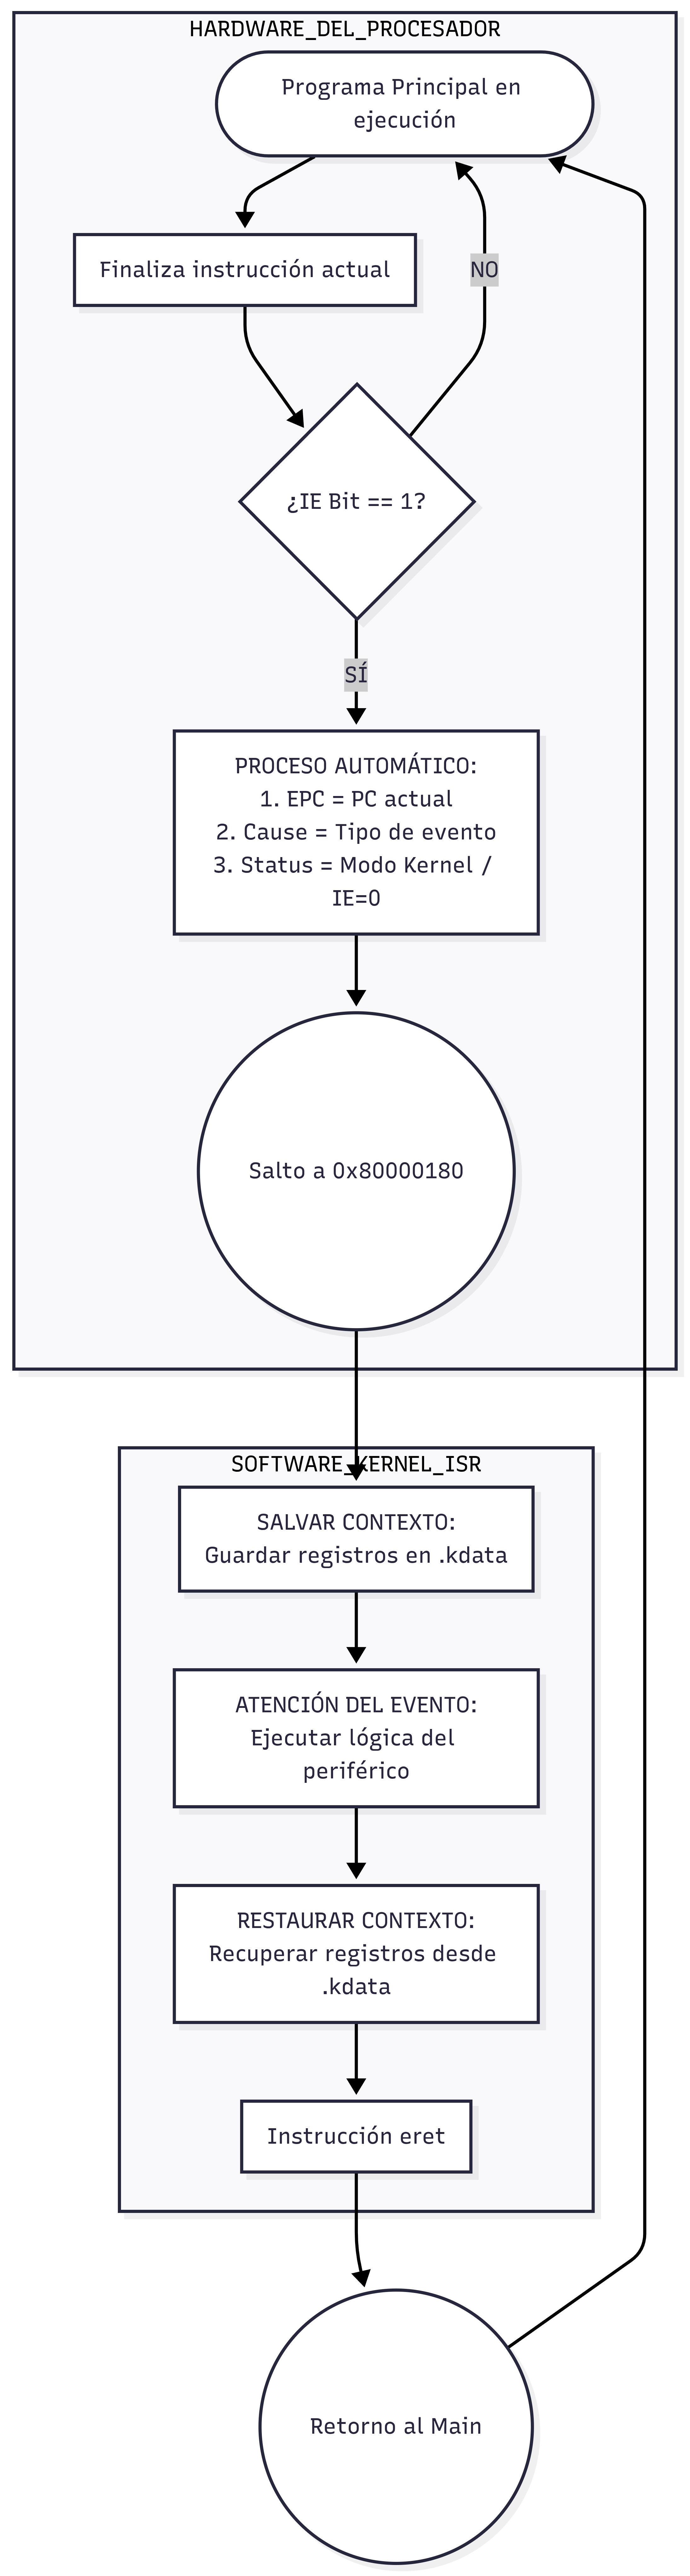
\includegraphics[width=0.4\textwidth]{Hardware-Software Execution-2026-03-10-020012.png} 
 \caption{Ciclo de vida de una interrupción de hardware.}
 \end{figure}
% -----------------------------------------

\subsubsection{2. ¿Qué diferencias hay entre gestionar E/S con sondeo y hacerlo con interrupciones?}

Por sondeo el procesador se centra solamente en preguntar directamente al hardware si esta listo, por lo que no puede ejecutar otra instrucción hasta que el hardware de la señal, desperdiciando millones de ciclos de reloj. Mientras que por interrupciones el hardware es el que le avisa al procesador que esta listo, lo cual es mucho mas eficiente ya que permite al procesador realizar otras tareas mientras el hardware da la señal.

\subsubsection{3. ¿Qué ventajas tiene el uso de interrupciones en términos de uso del procesador?}

El uso de interrupciones ofrece una mejora sustancial en el rendimiento del sistema al optimizar el uso del recurso más valioso: el tiempo de ejecución del procesador. Las principales ventajas son:

\begin{itemize}
    \item \textbf{Eliminación de la Espera Activa:} A diferencia del sondeo, donde el procesador consume ciclos de reloj innecesarios en un bucle cerrado consultando el hardware , las interrupciones permiten que el procesador se libere de esa carga.
    \item \textbf{Aprovechamiento de Recursos (Multitarea):} Al no tener que vigilar constantemente los periféricos, la CPU puede ejecutar otras tareas productivas o procesos de usuario mientras el hardware trabaja de forma independiente. Esto se observa en el ejercicio 1, donde el programa principal se dedica exclusivamente a medir el tiempo mientras el teclado funciona en segundo plano.
    \item \textbf{Reducción del Tiempo de Latencia:} El procesador puede reaccionar de forma casi inmediata ante eventos externos asíncronos. Esto garantiza una mayor fluidez en la interacción con el usuario, como ocurre en el ejercicio del semáforo, donde el cambio de estado se dispara en el instante exacto en que se presiona la tecla.
    \item \textbf{Ahorro de Energía:} En sistemas reales (especialmente dispositivos móviles), el procesador puede entrar en estados de bajo consumo o "sueño" y despertarse únicamente cuando un periférico genera una interrupción, lo que prolonga la vida útil de la batería.
\end{itemize}

\subsubsection{4. ¿Qué registros especiales se utilizan en MIPS32 para gestionar interrupciones?}

Para gestionar las interrupciones, la arquitectura MIPS32 utiliza los registros del Coprocesador 0 (CP0). Los tres registros más importantes son:

\begin{itemize}
    \item \textbf{Status (Registro 12):} Este registro controla el estado del procesador respecto a las interrupciones. Su función principal es actuar como un "panel de permisos". Contiene bits específicos para:
    \begin{itemize}
        \item \textbf{Interrupt Enable (IE):} Un bit global que habilita o deshabilita todas las interrupciones.
        \item \textbf{Interrupt Mask:} Varios bits que permiten habilitar o enmascarar (ignorar) interrupciones de dispositivos específicos (como el teclado o el reloj).
        \item \textbf{User/Kernel Mode:} Determina si el procesador está en modo de usuario (protegido) o en modo kernel (privilegiado).
    \end{itemize}
    \item \textbf{Cause (Registro 13):} Como su nombre indica, este registro registra la "causa" de la interrupción o excepción. Cuando el procesador salta a la rutina de servicio (0x80000180), el software lee este registro para saber qué ocurrió exactamente. Por ejemplo, permite distinguir si la interrupción fue causada por el teclado, por el temporizador, o si fue una excepción por un error matemático (división entre cero).
    \item \textbf{EPC - Exception Program Counter (Registro 14):} Es un registro de 32 bits que almacena la dirección de la instrucción que se estaba ejecutando en el programa principal en el momento exacto en que ocurrió la interrupción. Es vital para el retorno, ya que la instrucción eret toma el valor guardado en el EPC y lo devuelve al contador de programa (PC) para reanudar la ejecución normal.
\end{itemize}

\subsubsection{5. ¿Por qué es necesario guardar el contexto (registros) al entrar en una rutina de servicio?}

Guardar el contexto (que consiste en los valores de los registros que el procesador está utilizando en ese instante) es obligatorio debido a la naturaleza asíncrona de las interrupciones. Las razones principales son:

\begin{itemize}
    \item \textbf{Evitar la corrupción de datos:} Dado que una interrupción puede ocurrir en cualquier momento, el programa principal (main) seguramente está utilizando registros (como \$t0, \$at, o \$s0) para realizar cálculos o manejar direcciones. Si la Rutina de Servicio (ISR) utiliza esos mismos registros sin guardarlos primero, sobrescribirá los valores originales, provocando que el programa principal falle o produzca resultados incorrectos al retomar su ejecución.
    \item \textbf{Transparencia para el programa principal:} El objetivo de un sistema bien diseñado es que el programa interrumpido no "sepa" que fue pausado. Para lograr esto, el estado de la CPU al salir de la rutina de servicio debe ser idéntico al que tenía antes de entrar.
    \item \textbf{Gestión de registros compartidos:} En MIPS32, los registros de propósito general son recursos compartidos. Como la ISR es una función que se ejecuta de manera imprevista, no existe un acuerdo previo entre el main y la ISR sobre qué registros están "libres". Por lo tanto, la ISR asume la responsabilidad total de respaldar cualquier registro que planee utilizar en una zona de memoria segura (como el segmento .kdata).
\end{itemize}

\subsubsection{6. Momentos en que pueden generarse excepciones en un sistema MIPS32}

\textbf{a) Situaciones que generan una excepción:} En la arquitectura MIPS32, las excepciones pueden dispararse por diversas causas internas al flujo de instrucciones:
\begin{itemize}
    \item \textbf{Desbordamiento aritmético (Arithmetic Overflow):} Ocurre cuando el resultado de una operación aritmética excede el rango representable del registro de destino (por ejemplo, al sumar dos números muy grandes con la instrucción add).
    \item \textbf{Fallo de dirección (Address Error):} Se genera cuando se intenta acceder a una dirección de memoria que no está correctamente alineada (como intentar leer una palabra de 32 bits en una dirección que no es múltiplo de 4) o cuando se intenta acceder a una dirección fuera del rango permitido.
    \item \textbf{Instrucción no definida (Reserved Instruction):} El procesador encuentra un código de operación (opcode) que no reconoce como una instrucción válida de su conjunto de instrucciones.
    \item \textbf{Llamada al sistema (System Call):} Aunque es intencional, la instrucción syscall genera una excepción para transferir el control al sistema operativo y solicitar un servicio (como imprimir en consola).
    \item \textbf{Breakpoint:} Utilizada principalmente para depuración (debugging), detiene la ejecución del programa y transfiere el control al depurador.
\end{itemize}

\textbf{b) Etapas del pipeline que pueden provocar una excepción:} El procesador MIPS32 utiliza un pipeline de 5 etapas (IF, ID, EX, MEM, WB). Casi todas las etapas, excepto el "Write Back", pueden ser el origen de una excepción debido a su función específica:
\begin{itemize}
    \item \textbf{IF (Instruction Fetch):} Puede provocar excepciones por fallos en el acceso a la memoria de instrucciones o errores de alineación al intentar obtener la siguiente instrucción.
    \item \textbf{ID (Instruction Decode):} Es donde se detectan las instrucciones no definidas o inválidas, disparando la excepción correspondiente antes de que la instrucción pase a ejecución.
    \item \textbf{EX (Execution):} En esta etapa es donde la Unidad Aritmético Lógica (ALU) detecta el desbordamiento aritmético (overflow) tras realizar un cálculo.
    \item \textbf{MEM (Memory Access):} Similar a la etapa IF, pero aplicada a los datos. Aquí se generan excepciones por fallos de dirección o alineación al intentar ejecutar instrucciones de carga (lw) o almacenamiento (sw).
\end{itemize}

\subsubsection{7. Estrategias de tratamiento de excepciones e interrupciones}

\textbf{a) Diferencias entre interrupciones y excepciones:} Aunque ambas desvían el flujo del programa hacia el Kernel, su origen y naturaleza son distintos:
\begin{itemize}
    \item \textbf{Excepciones (Síncronas):} Son eventos internos generados por la propia ejecución de las instrucciones del programa. Se consideran síncronas porque ocurren en un momento predecible: justo cuando se intenta ejecutar la instrucción que causa el error (como una división por cero o un desbordamiento).
    \item \textbf{Interrupciones (Asíncronas):} Son eventos externos provocados por dispositivos de hardware ajenos al flujo del procesador (como el teclado o un disco duro). Se consideran asíncronas porque pueden ocurrir en cualquier instante, sin ninguna relación directa con la instrucción que se esté ejecutando en ese momento.
\end{itemize}

\textbf{b) Estrategias y redirección:} Existen dos formas principales en las que un procesador puede decidir a dónde saltar cuando ocurre uno de estos eventos:
\begin{itemize}
    \item \textbf{Interrupciones Vectoreadas:} El hardware tiene una tabla con diferentes direcciones de memoria para cada tipo de evento. Si falla el reloj, salta a una dirección; si falla el teclado, salta a otra. Esto es muy rápido pero requiere más hardware.
    \item \textbf{Manejador Único (No vectoreada):} Es la que usa MIPS32 por defecto. Todos los eventos, sin importar la causa, redirigen la ejecución a una única dirección fija (típicamente 0x80000180). Una vez allí, el software debe leer el registro Cause para identificar qué pasó y decidir qué hacer.
\end{itemize}
Cuando se detecta el evento, el hardware del procesador realiza un "salto forzado" automático. Cambia el contador de programa (PC) a la dirección de excepción (0x80000180) y eleva el nivel de privilegio del procesador a modo Kernel, permitiendo el acceso a recursos protegidos. 

\textbf{Función del registro EPC:} El EPC actúa como un "marcapáginas" de seguridad. Su función es almacenar la dirección de memoria de la instrucción que estaba siendo ejecutada (en el caso de una interrupción) o de la instrucción que causó el error (en el caso de una excepción). Sin este registro, el procesador no tendría forma de saber a dónde regresar para continuar con el programa principal tras ejecutar la instrucción eret.

\subsubsection{8. Habilitación de interrupciones en dispositivos y procesador}

\textbf{a) Procedimiento de habilitación:}
\begin{itemize}
    \item \textbf{En el Teclado:} Se debe acceder al Registro de Control del Teclado, ubicado en la dirección de memoria 0xFFFF0000. Específicamente, se debe poner en 1 el bit 1 (Interrupt Enable) de este registro. En ensamblador, esto se logra leyendo el valor actual, aplicando una máscara OR con el valor 2 y guardando el resultado de vuelta.
    \item \textbf{En la Pantalla (Display):} De manera análoga al teclado, se debe acceder al Registro de Control del Transmisor, ubicado en la dirección 0xFFFF0008. Se debe activar el bit 1 para permitir que la pantalla genere una interrupción cada vez que esté lista para mostrar un nuevo carácter.
    \item \textbf{En el Procesador (Registro Status):} Se deben modificar dos áreas críticas del registro Status (Registro 12 del Coprocesador 0):
    \begin{itemize}
        \item \textbf{Bit 0 (IE - Interrupt Enable):} Es el interruptor maestro global. Si este bit es 0, todas las interrupciones están deshabilitadas.
        \item \textbf{Bits 8 al 15 (IM - Interrupt Mask):} Estos bits actúan como filtros individuales para cada nivel de interrupción. Para que el teclado funcione, el bit correspondiente a su nivel de hardware (usualmente el bit 9 o 11 dependiendo de la configuración de MARS) debe estar en 1.
    \end{itemize}
\end{itemize}

\textbf{b) Habilitación parcial:} Si habilitamos las interrupciones en los dispositivos (poniendo a 1 el bit de control en 0xFFFF0000) pero no en el procesador (manteniendo el bit IE en 0), ocurriría lo siguiente: El periférico detectará el evento (la pulsación de una tecla) y enviará una señal eléctrica de interrupción hacia el procesador. Sin embargo, el procesador, al tener su "llave maestra" apagada, ignorará la señal por completo. El programa principal continuará ejecutándose como si nada hubiera pasado y el evento de hardware se perderá o quedará pendiente sin ser atendido hasta que el procesador decida habilitar sus interrupciones.

\subsubsection{9. Procesamiento de interrupciones}

Cuando se produce una interrupción de reloj (timer interrupt), el sistema sigue una secuencia estrictamente coordinada entre el hardware y el software:

\textbf{Fase 1: Acción del Hardware (Automática)}
\begin{itemize}
    \item \textbf{Evento:} El temporizador de hardware alcanza el valor comparador y envía una señal eléctrica al procesador.
    \item \textbf{Detección:} El procesador termina la instrucción actual y verifica que las interrupciones estén habilitadas en el registro Status.
    \item \textbf{Resguardo de Emergencia:} El hardware copia automáticamente el valor actual del PC al registro EPC y registra el código de la interrupción en el registro Cause.
    \item \textbf{Cambio de Modo:} El procesador cambia a 'Modo Kernel' y deshabilita nuevas interrupciones para evitar conflictos iniciales.
    \item \textbf{Salto:} Se carga la dirección 0x80000180 en el contador de programa (PC), forzando el inicio de la Rutina de Servicio (ISR).
\end{itemize}

\textbf{Fase 2: Acción del Software (La Rutina de Servicio)}
\begin{itemize}
    \item \textbf{Salvaguarda del Contexto:} La rutina guarda en el segmento .kdata o en la pila los registros que planea utilizar, como \$at, \$t0, \$t1, etc., para no destruir los datos del programa de usuario.
    \item \textbf{Identificación:} El software lee el registro Cause para confirmar que la interrupción fue efectivamente de reloj.
    \item \textbf{Procesamiento:} Se realiza la tarea programada (por ejemplo, actualizar un contador de milisegundos o verificar si han pasado los 20 segundos del ejercicio).
    \item \textbf{Restauración:} Se recuperan los valores originales de los registros desde la memoria hacia el banco de registros.
    \item \textbf{Retorno:} Se ejecuta la instrucción eret, que devuelve al procesador al modo usuario y restaura el PC desde el EPC.
\end{itemize}

\textbf{Importancia de guardar el contexto:} Es crítico guardar los registros generales, el EPC y el Status por las siguientes razones:
\begin{itemize}
    \item \textbf{Registros Generales (\$at, \$t0, etc.):} Al ser una interrupción asíncrona, el programa de usuario no sabe que ha sido pausado. Si la rutina modifica un registro que el usuario estaba usando para un cálculo, al volver, los datos estarán corruptos.
    \item \textbf{EPC:} Si ocurriera una segunda interrupción (o una excepción) dentro de la primera sin haber guardado el EPC anterior, la dirección de retorno al programa principal se perdería para siempre, causando el colapso del sistema.
    \item \textbf{Registro Status:} Este registro contiene los permisos y el modo de operación (Usuario/Kernel). Al restaurarlo, nos aseguramos de que el procesador vuelva al estado de privilegios correcto que tenía el usuario antes de la interrupción.
\end{itemize}

\subsubsection{10. Interrupciones de reloj y control de ejecución}

\textbf{a) Uso de la interrupción de reloj para el control de procesos}
\begin{itemize}
    \item \textbf{Evitar bucles infinitos:} El SO no confía ciegamente en que un programa terminará por sí solo. Antes de darle el control de la CPU a un programa, el SO configura un temporizador (como un "reloj de arena" de hardware). Si el programa cae en un bucle infinito, la interrupción de reloj se disparará eventualmente, devolviendo el control al Kernel (ISR) de forma forzada y permitiendo al SO retomar el mando.
    \item \textbf{Finalizar programas por tiempo máximo (Timeouts):} En sistemas de tiempo compartido o servidores, se asigna a cada programa un "cuanto" de tiempo (time slice). Cuando la interrupción de reloj notifica que el tiempo asignado ha expirado, el planificador del sistema operativo (scheduler) puede decidir suspender o finalizar el programa para permitir que otros procesos utilicen el procesador.
\end{itemize}

\textbf{b) Finalización anticipada del programa:} Si un programa finaliza su ejecución de manera exitosa antes de que ocurra la interrupción de reloj programada, el software (el sistema operativo) debe realizar las siguientes acciones de limpieza:
\begin{itemize}
    \item \textbf{Desactivar el temporizador:} El Kernel debe cancelar o resetear la solicitud de interrupción pendiente en el hardware para evitar que se dispare una interrupción innecesaria sobre un proceso que ya no existe en la memoria.
    \item \textbf{Liberar recursos:} El sistema debe limpiar los registros especiales relacionados con ese proceso (como el EPC o el estado en el registro Status) y liberar la memoria asignada.
    \item \textbf{Actualizar el planificador:} El SO marca al procesador como "disponible" de inmediato para que el siguiente proceso en la cola pueda comenzar a ejecutarse, optimizando así el rendimiento global del sistema.
\end{itemize}

\subsubsection{11. Análisis y Discusión de los Resultados}

Tras la implementación de los ejercicios de gestión de entrada/salida mediante interrupciones en el simulador MARS, se extraen las siguientes conclusiones técnicas:

Se validó que el uso de interrupciones permite al procesador ejecutar tareas productivas en el programa principal (main) mientras espera eventos externos. En el Ejercicio 1, el procesador pudo mantener un conteo preciso de 20 segundos mediante syscall 30 sin verse afectado por la entrada de datos, demostrando que la atención al teclado solo consume ciclos de CPU cuando es estrictamente necesario. Esto representa una mejora crítica de rendimiento respecto al modelo de sondeo (polling) de la práctica anterior, donde la CPU quedaba bloqueada en bucles de espera activa.

La implementación del buffer circular demostró ser una solución eficaz para el manejo de flujos de datos continuos, permitiendo que el índice de escritura regrese a cero al alcanzar el límite de memoria sin desbordar el segmento de datos. Además, se comprobó la importancia del Coprocesador 0 y la dirección fija 0x80000180 como el punto de entrada universal para el manejo de excepciones y eventos de hardware en MIPS32.

El Ejercicio 3 (Semáforo) ilustró el uso exitoso de variables de control o "flags" para la comunicación entre el Kernel y el Usuario. Al delegar solo el cambio de la bandera (flag\_pulsador) a la interrupción, se garantizó que la rutina de servicio fuera breve y eficiente, evitando el uso de llamadas al sistema pesadas dentro del segmento .ktext. Se verificó que las transiciones de estado (20s, 10s y 30s) ocurren de manera determinista una vez que la interrupción asíncrona altera el flujo del bucle de espera en el main.

Finalmente, la correcta utilización del segmento .kdata para respaldar registros como \$at, \$t0 y \$t1 fue vital para la estabilidad del sistema. Durante las pruebas, se observó que cualquier omisión en el resguardo de estos registros provocaba un comportamiento errático o el cierre inesperado del programa principal, confirmando que la transparencia para el usuario depende de una restauración meticulosa del estado del procesador tras el eret.

\section{Anexos}

\subsection{Rutina de Servicio de Interrupción: Buffer de Teclado (Ejercicio 1)}

\begin{lstlisting}[language=mips]
##################################################
# RUTINA DE SERVICIO DE INTERRUPCION (ISR)
##################################################
.ktext 0x80000180
    
    # 1. Salvar el contexto (Guardar registros)
    .set noat               
    sw $at, save_at
    .set at
    sw $t0, save_t0
    sw $t1, save_t1
    sw $t2, save_t2
    sw $t3, save_t3

    # 2. Leer la tecla pulsada
    li $t0, 0xFFFF0000      
    lw $t2, 4($t0)          # Leemos el codigo ASCII desde 0xFFFF0004

    # 3. Filtro de mayusculas (ASCII 65 al 90)
    blt $t2, 65, salir_interrupcion  
    bgt $t2, 90, salir_interrupcion  

    # 4. Guardar en el buffer circular
    lw $t1, buf_w           # Cargar indice de escritura
    la $t0, buffer          
    add $t0, $t0, $t1       
    sb $t2, 0($t0)          # Escribir la letra en buffer[buf_w]

    # Calcular siguiente posicion de escritura
    addi $t1, $t1, 1
    blt $t1, 100, no_wrap_w
    li $t1, 0               # Si llega a 100, vuelve a 0 (Circular)
no_wrap_w:
    
    # Verificar si el buffer esta lleno (escritura alcanzo a lectura)
    lw $t3, buf_r
    bne $t1, $t3, guardar_w
    
    # Si esta lleno, empujamos el indice de lectura (sobrescribimos lo viejo)
    addi $t3, $t3, 1
    blt $t3, 100, no_wrap_r_isr
    li $t3, 0
no_wrap_r_isr:
    sw $t3, buf_r           # Guardamos el nuevo indice de lectura

guardar_w:
    sw $t1, buf_w           # Guardamos el nuevo indice de escritura

salir_interrupcion:
    # 5. Restaurar el contexto
    .set noat
    lw $at, save_at
    .set at
    lw $t0, save_t0
    lw $t1, save_t1
    lw $t2, save_t2
    lw $t3, save_t3

    # 6. Retornar al programa principal
    eret
\end{lstlisting}

\subsection{Rutina de Servicio de Interrupción: Semáforo (Ejercicio 3)}

\begin{lstlisting}[language=mips]
##################################################
# RUTINA DE SERVICIO DE INTERRUPCION (ISR)
##################################################
.ktext 0x80000180

    # 1. Salvar el contexto (Guardar registros)
    .set noat
    sw $at, save_at
    .set at
    sw $t0, save_t0
    sw $t1, save_t1

    # 2. Leer la tecla que causo la interrupcion
    li $t0, 0xFFFF0000
    lw $t1, 4($t0)

    # 3. Filtrar si la tecla fue s (minuscula)
    bne $t1, 115, salir_interrupcion # si no es la 's', ignorar y salir

    # 4. Si fue la 's': encender la bandera 
    li $t1, 1
    sw $t1, flag_pulsador

salir_interrupcion:
    # 5. Restaurar contexto y regresar
    .set noat
    lw $at, save_at
    .set at
    lw $t0, save_t0
    lw $t1, save_t1
    
    # 6. Retornar al programa principal
    eret
\end{lstlisting}

\end{document}